\documentclass{exam}
\usepackage[utf8]{inputenc}
\usepackage{lmodern}
\usepackage{microtype}

% \usepackage[parfill]{parskip}
\usepackage[dvipsnames]{xcolor}
\usepackage{amsmath}
\usepackage{amsfonts}
\usepackage{amsthm}
\usepackage{siunitx}
\DeclareSIUnit\year{yr}
\DeclareSIUnit\foot{ft}
\DeclareSIUnit\litre{\liter}

\usepackage{skull}

\usepackage{pgfplots}
\usepgfplotslibrary{polar}
\pgfplotsset{compat=1.11}
\usepgfplotslibrary{statistics}
\usepackage{graphicx}
\usepackage{sidecap}
\sidecaptionvpos{figure}{c}
\usepackage{float}
\usepackage{gensymb}
\usepackage{tkz-euclide}
\usetkzobj{all}
\usepackage{commath}
\usepackage{hyperref}
\usepackage{enumitem}
\usepackage{wasysym}
\usepackage{multicol}
\usepackage{mathtools}
\usepackage{tcolorbox}
\usepackage{tabularx}
\usepackage[version=4]{mhchem}
\usepackage{changepage}
\usepackage{listings}
\lstset{basicstyle=\ttfamily\linespread{0.8}\small}

\renewcommand*{\thefootnote}{\fnsymbol{footnote}}

\newtheorem*{thm}{Theorem}
\newtheorem*{iden}{Identity}
\newtheorem*{lemma}{Lemma}
\newtheorem{obs}{Observation}
\theoremstyle{definition}
\newtheorem*{defn}{Definition}
\newtheorem*{ex}{Example}
\newtheorem{con}{Construction}
\newtheorem*{alg}{Algorithm}

\newtheoremstyle{break}
  {\topsep}{\topsep}%
  {\itshape}{}%
  {\bfseries}{}%
  {\newline}{}%
\theoremstyle{break}
\newtheorem*{bthm}{Theorem}

% russian integral
\usepackage{scalerel}
\DeclareMathOperator*{\rint}{\scalerel*{\rotatebox{17}{$\!\int\!$}}{\int}}

% \DeclareMathOperator*{\rint}{\int}

\pgfplotsset{vasymptote/.style={
    before end axis/.append code={
        \draw[densely dashed] ({rel axis cs:0,0} -| {axis cs:#1,0})
        -- ({rel axis cs:0,1} -| {axis cs:#1,0});
    }
}}

% \pointsinrightmargin
\boxedpoints
\pointname{}

\newcommand{\questioA}{\question[\texttt{\textbf{\color{Cerulean} A}}]}
\newcommand{\questioM}{\question[\texttt{\textbf{\color{PineGreen} M}}]}
\newcommand{\questioE}{\question[\texttt{\textbf{\color{WildStrawberry} E}}]}
\newcommand{\questioS}{\question[\texttt{\textbf{\color{Goldenrod} S}}]}
\newcommand{\questioO}{\question[\texttt{\textbf{\color{BurntOrange} O}}]}

\newcommand{\parA}{\part[\texttt{\textbf{\color{Cerulean} A}}]}
\newcommand{\parM}{\part[\texttt{\textbf{\color{PineGreen} M}}]}
\newcommand{\parE}{\part[\texttt{\textbf{\color{WildStrawberry} E}}]}
\newcommand{\parS}{\part[\texttt{\textbf{\color{Goldenrod} S}}]}
\newcommand{\parO}{\part[\texttt{\textbf{\color{BurntOrange} O}}]}

\newcommand{\subparA}{\subpart[\texttt{\textbf{\color{Cerulean} A}}]}
\newcommand{\subparM}{\subpart[\texttt{\textbf{\color{PineGreen} M}}]}
\newcommand{\subparE}{\subpart[\texttt{\textbf{\color{WildStrawberry} E}}]}
\newcommand{\subparS}{\subpart[\texttt{\textbf{\color{Goldenrod} S}}]}
\newcommand{\subparO}{\subpart[\texttt{\textbf{\color{BurntOrange} O}}]}

\newcommand{\mainHeader}[2]{\section*{NCEA Level 2 Mathematics\\#1. #2}}
\newcommand{\mainHeaderHw}[2]{\section*{NCEA Level 2 Mathematics (Homework)\\#1. #2}}
\newcommand{\seealso}[1]{\begin{center}\emph{See also #1.}\end{center}}
\newcommand{\drills}[1]{\begin{center}\emph{Drill problems: #1.}\end{center}}
\newcommand{\basedon}[1]{\begin{center}\emph{Notes largely based on #1.}\end{center}}

\begin{document}

\mainHeaderIntg{16}{Anti-differentiation}
For some time, we have been hinting that finding area was in some way the inverse to finding slope. In last
week's questions, the curtain was pulled back a little further when we calculated an area function for a variable endpoint, took
the derivative, and got the original function back. Next week, all will be revealed; but first, we need to do a little bit more
work. This week, we're going to look at \textbf{anti-differentiation}: finding the original function given its derivative.

\begin{ex}
  One antiderivative of $ y' = 3x^2 + 4 $ is $ x^3 + 4x $. Another is $ x^3 + 4x + 1 $. A third is $ x^3 + 4x + 7 $. Obviously
  every function of the form $ y = x^3 + 4x + C $ for some constant $ C $ will differentiate to the given $ y' $, so we must remember
  always to make this clear.
\end{ex}

We also call antiderivatives \textbf{indefinite integrals}, and in this notation the above example is
\begin{displaymath}
  \rint 3x^2 + 4 \dif{x} = x^3 + 4x + C.
\end{displaymath}

Unfortunately, there is no `easy' way to anti-differentiate; we simply have to try to rearrange the function in some clever
way until it looks like something that we know how to deal with.

\begin{joke}
  Two mathematicians are in a bar. The first one says to the second that the average person knows very little about basic
  mathematics. The second one disagrees and claims that most people can cope with a reasonable amount of maths. The first
  mathematician goes off to the washroom, and in his absence the second calls over the waitress. He tells her that in a few
  minutes, after his friend has returned, he will call her over and ask her a question. All she has to do is answer ``one
  third $x$ cubed.'' She repeats ``one thir–dex cue?'' He repeats ``one third $x$ cubed.'' She asks, ``one thir dex cuebd?'' “Yes,
  that’s right,” he says. So she agrees, and goes off mumbling to herself, ``one thir dex cuebd...''. The first guy returns
  and the second proposes a bet to prove his point, that most people do know something about basic math. He says he will ask
  the blonde waitress an integral, and the first laughingly agrees. The second man calls over the waitress and asks ``what is
  the integral of $x$ squared?'' The waitress says ``one third $x$ cubed'' and while walking away, turns back and says over
  her shoulder, ``plus a constant!''
\end{joke}

\begin{exs}\leavevmode
  \begin{enumerate}
    \item The most general antiderivative of $ \sin x $ is $ -\cos x + C $.
    \item The most general antiderivative of $ \tan x $ is $ -\ln \abs{\cos x} + C $.
    \item $ \rint \frac{1}{x + 3} \dif{x} = \ln \abs{x + 3} + C $.
    \item $ \rint \tan^2 \theta \dif{\theta} = \rint \sec^2 \theta - 1 \dif{\theta} = \tan \theta - \theta + C $.
    \item $ \rint \frac{2x}{x^2 + 1} \dif{x} = \ln \abs{x^2 + 1} + C $.
    \item $ \rint Ke^{Kx} \dif{x} = e^{Kx} + C $ for all constants $ K $.
  \end{enumerate}
\end{exs}

\subsection*{Questions}
\begin{questions}
  \questioA For each expression, find the most general antiderivative with respect to $ x $.
    \begin{multicols}{2}
    \begin{parts}
      \part $ 2x $
      \part $ x^{-3} $
      \part $ 0 $
      \part $ \sec^2 x + \sqrt{x} $
      \part $ x\sqrt{x} $
      \part $ \sin x - \cos x $
      \part $ \frac{2x^3 + 3x - \sqrt{x}}{\sqrt[3]{x}} $
      \part $ \frac{1}{x^2} + e^x $.
    \end{parts}
    \end{multicols}
  \questioA Verify the examples in the notes by differentiation.
  \questioA Show that $ \rint 3x^2 + 4x + 5 + 2e^{2x} \dif{x} = x^3 + 2x^2 + 5x + e^{2x} + C $.
  \questioA Find $ y' $ when $ y = 3 + \sin (2x + 4) $ and hence find $ \rint 2 \cos(2x + 4) \dif{x} $.
  \questioA If $ \od{y}{t} = 1.5 \sqrt{t} $ and $ y(4) = 10 $, find $ y(t) $ exactly.
  \questioM Find $ f $ if $ f''(x) = 12x^2 + 6x - 4 $, $ f(0) = 4 $, $ f(1) = 1 $.
  \questioA The velocity of a particle is given by $ v(t) = 2t + 1 $. Find its position at $ t = 4 $
            if its position at $ t = 0 $ is $ x = 0 $.
  \questioM The acceleration of a particle is given by $ a(t) = 10\sin t + 3\cos t $. At $ t = 0 $, its position is $ x = 0 $; at $ t = 2\pi $,
            its position is $ x = 12 $. Find its position at $ t = \frac{\pi}{2} $.
  \questioA Find all functions $ g $ such that $ g'(x) = 4 \sin x + \frac{2x^5 - \sqrt{x}}{x} $.
  \questioM For each function, sketch an antiderivative passing through $ (0, 0) $:
            \begin{center}
              \begin{tabular}{ccc}
                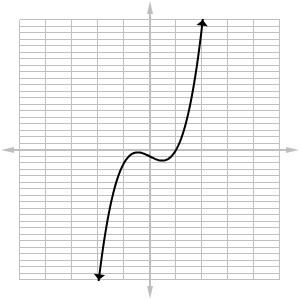
\includegraphics[width=0.28\textwidth]{anti1}&
                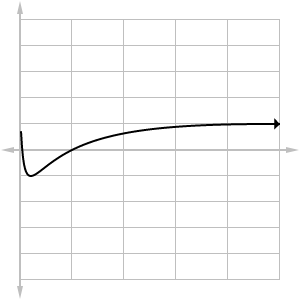
\includegraphics[width=0.28\textwidth]{anti2}&
                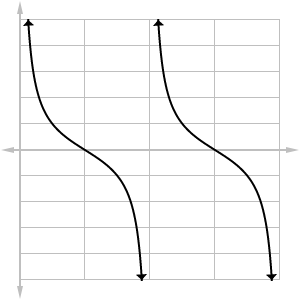
\includegraphics[width=0.28\textwidth]{anti3}\\
                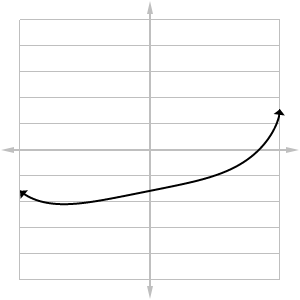
\includegraphics[width=0.28\textwidth]{anti4}&
                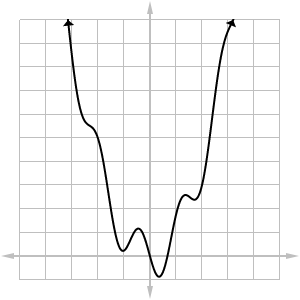
\includegraphics[width=0.28\textwidth]{anti5}&
                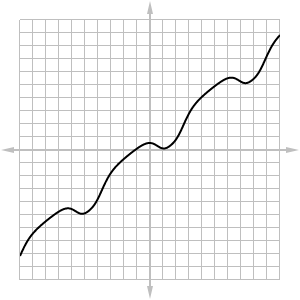
\includegraphics[width=0.28\textwidth]{anti6}
              \end{tabular}
            \end{center}
  \questioE Show that if $ F $ is an anti-derivative of $ f $, $ G $ is an anti-derivative of $ g $, and $ \alpha $ and $ \beta $ are any constants,
            then $ \alpha F + \beta G $ is an anti-derivative of $ \alpha f + \beta g $.
  \questioE Give an example of functions $ f $ and $ g $ such that if $ F $ and $ G $ are anti-derivatives of $ f $ and $ g $ respectively then $ FG $
            is \emph{not} an anti-derivative of $ fg $.
  \questioE Note that on the formula sheet, the anti-derivative of $ 1/x $ is given as $ \ln \abs{x} $, not just $ \ln x $.
    \begin{parts}
      \part Compute $ \od{}{x} \ln \abs{x} $ if $ x < 0 $, and hence justify formally why $ \od{}{x} \ln \abs{x} = 1/x $.
      \part Draw $ y = \ln \abs{x} $ and $ y = 1/x $ on the same pair of axes, and hence justify intuitively why $ \od{}{x} \ln \abs{x} = 1/x $.
    \end{parts}
\end{questions}

\end{document}
